%
% IEEE Transactions on Microwave Theory and Techniques example
% Tibault Reveyrand - http://www.microwave.fr
%
% http://www.microwave.fr/LaTeX.html
% ---------------------------------------



% ================================================
% Please HIGHLIGHT the new inputs such like this :
% Text :
%  \hl{comment}
% Aligned Eq. 
% \begin{shaded}
% \end{shaded}
% ================================================

\documentclass[journal]{IEEEtran}

%\usepackage[retainorgcmds]{IEEEtrantools}
%\usepackage{bibentry}  
\usepackage{xcolor,soul,framed} %,caption

\colorlet{shadecolor}{yellow}
% \usepackage{color,soul}
\usepackage[pdftex]{graphicx}
\graphicspath{{../pdf/}{../jpeg/}}
\DeclareGraphicsExtensions{.pdf,.jpeg,.png}

\usepackage[cmex10]{amsmath}
%Mathabx do not work on ScribTex => Removed
%\usepackage{mathabx}
\usepackage{array}
\usepackage{mdwmath}
\usepackage{mdwtab}
\usepackage{eqparbox}
\usepackage{url}

\hyphenation{op-tical net-works semi-conduc-tor}

%\bstctlcite{IEEE:BSTcontrol}


%=== TITLE & AUTHORS ====================================================================
\begin{document}
\bstctlcite{IEEEexample:BSTcontrol}
    \title{How can the effectiveness of marketing ‘Airbnb Seattle’ be improved?
– dataset of 2016 
}
  \author{LIST Nicole ,
      LÖHR Tim,\\
      BOHNSTEDT Timo,
      PANG Tsz Ching,
      and~BAL Kiran Jeniffer% <-this % stops a space
      
      

  \thanks{Manuscript received July 10, 2012. \hl{This paper is an expanded paper from the IEEE MTT-S Int. Microwave Symposium held on June 17-22, 2012 in Montreal, Canada.} This work was funded in part by the Office of Naval Research under the Defense Advanced Research Projects Agency (DARPA) Microscale Power Conversion (MPC) Program under Grant N00014-11-1-0931, and in part by the Advanced Research Projects Agency-Energy (ARPA-E), U.S. Department of Energy, under Award Number DE-AR0000216.}
  \thanks{M. Roberg is with TriQuint Semiconductor, 500 West Renner Road Richardson, TX 75080 USA (e-mail: michael.roberg@tqs.com).}% <-this % stops a space
  \thanks{T. Reveyrand is with the XLIM Laboratory, UMR 7252, University of Limoges, 87060 Limoges, France (e-mail: tibault.reveyrand@xlim.fr).}%
  \thanks{I. Ramos and Z. Popovic are with the Department of Electrical, Computer and Energy Engineering, University of Colorado, Boulder, CO, 80309-0425 USA (e-mail: ignacio.ramos@colorado.edu; zoya.popovic@colorado.edu).}% <-this % stops a space
  \thanks{E. Falkenstein is with Qualcomm Inc., 6150 Lookout Road
Boulder, CO 80301 USA (e-mail: erez.falkenstein@gmail.com).}}  


% The paper headers
\markboth{Project Report
Machine Learning for Business IS4861 
}{Roberg \MakeLowercase{\textit{et al.}}: High-Efficiency Diode and Transistor Rectifiers}


% ====================================================================
\maketitle



% === ABSTRACT ====================================================================
% =================================================================================
\begin{abstract}
%\boldmath
This paper presents a theoretical analysis of harmonically-terminated high-efficiency power rectifiers and experimental validation on a class-C single Schottky-diode rectifier and a class-F$^{\rm -1}$ GaN transistor rectifier. The theory is based on a Fourier analysis of current and voltage waveforms which arise across the rectifying element when different harmonic terminations are presented at its terminals. An analogy to harmonically-terminated power amplifier theory is discussed. From the analysis, one can obtain an optimal value for the DC load given the RF circuit design. An upper limit on rectifier efficiency is derived for each case as a function of the device on-resistance. Measured results from fundamental frequency source-pull measurement of a Schottky diode rectifier with short-circuit terminations at the second and third harmonic are presented. A maximal device rectification efficiency of 72.8\% at 2.45\,GHz matches the theoretical prediction. A 2.14\,GHz GaN pHEMT rectifier is designed based on a class-F$^{\rm -1}$ power amplifier. The gate of the transistor is terminated in an optimal impedance for self-synchronous rectification. Measurements of conversion efficiency and output DC voltage for varying gate RF impedance, DC load and gate bias are shown with varying input RF power at the drain. The rectifier demonstrates an efficiency of 85\% for a 10\,W input RF power at the transistor drain, with a DC voltage of \hl{30\,V} across a 98\,$\Omega$ resistor.
\end{abstract}


% === KEYWORDS ====================================================================
% =================================================================================
\begin{IEEEkeywords}
\hl{kaggle, machine learning, business, data analytics, airbnb}
\end{IEEEkeywords}






% For peer review papers, you can put extra information on the cover
% page as needed:
% \ifCLASSOPTIONpeerreview
% \begin{center} \bfseries EDICS Category: 3-BBND \end{center}
% \fi
%
% For peerreview papers, this IEEEtran command inserts a page break and
% creates the second title. It will be ignored for other modes.
\IEEEpeerreviewmaketitle


% ====================================================================
% ====================================================================
% ====================================================================











% === I. INTRODUCTION =============================================================
% =================================================================================
\section{Project background and motivation}

\IEEEPARstart{T}{he} dataset we are going to analyze contains several information about the renting of apartments via the platform Airbnb in Seattle. By analyzing the data, we want to find possibilities to improve the marketing of Airbnb optimized for Seattle. Mentioning the word ‘marketing’ most people immediately think about advertisement. Indeed, this is a very important part of marketing but it is far not enough to cover the whole meaning of marketing. By definition it rather is about the firm’s effort to address customer needs as well as their expectation and to orient their products according to the requirements of customers. So, it is also about the tradeoff of ‘evoking’ needs and expectation of consumers on a level that the product can satisfy and is able to compete with competitive products. To fulfill this, applying marketing instruments like the marketing mix can be helpful. The marketing mix consists of four policies: Product, Price, Promotion and Place. In the following the tasks and aims arising in these four areas will be described and explained how our data analysis can help to improve tasks in these areas aiming for a better overall marketing.\\As Airbnb is an agent for lessors, who want to rent their apartment to tourists, it ears its money by receiving a commission for every rented apartment. Therefore, Airbnb should aim for a high booking rate to increase their own profit. That is one reason, why Airbnb should care which apartments are offered on their platform and how they are presented (e.g. by the description, price, …). So, it can make sense for Airbnb to give lessors some suggestions how to promote and present their accommodation to achieve a maximal booking rate. Deducted of this assumption, we want to provide some suggestions for lessors to promote their apartments in the perfect manner but also want to give some suggestions, what point in time is best for Airbnb to release a marketing campaign to advertise some apartments in Seattle. 
\subsection{Product}
\noindent As already mentioned before, marketing is about fulfilling customer needs and expectations. Within product policy the aim is to understand one’s market and be able to figure out which needs and wants the customers have. In general, one can say that the main need of travelers is to find an accommodation but nowadays it is not only about finding accommodations but even more about discovering the right accommodation. It is not only having a nice and clean room bathroom, with white and clean towels and bead sheets. The surrounding and flair of the accommodation becomes more and more important. This issue Airbnb has already addressed in its advertising spot , so Airbnb is aware of the wants of travelers and is responsive to this in its advertisement. Thinking a step further, it is not enough to just show the customer that renting Airbnb apartments is a nice way to ‘really live’ there instead of just ‘go there’. When the customer has been attracted by Airbnb to search for on apartment on their website it is important to present the apartment in a good way. Therefore, the description of the apartments should mention all aspects the customer considers as important. By our data analysis we would like to support the lessor in creating a good and appealing description. By analyzing the reviews of customers and filtering the 50 most mentioned words, we can conclude that these mentioned words are important to customers and therefore lessors should mention them in their description. As Seattle is a huge city with lots of different areas with different style and flairs, we conduct word clouds for every neighborhood. This offers the advantage that we can better address and select certain customer groups. A neighborhood, with lots of parks, is probably better for nature lover than for reveler. So, nature lovers will mention the parks in their reviews very often and according to our word cloud (which is based on the reviews), lessors in this neighborhood will focus on the parks around their accommodation. If a person, who prefers partying at night, reads this description his or her interest will not be raised and therefore the person will search for apartments in another neighborhood. This creates and ‘automatic’ selection and increase the chance that a customer finds an apartment in a neighborhood, which fits his/ her interest. So, a first question we would like to answer is: Which facts lessors need to address in their description to raise the interest of potential customer, who ‘fit’ the vibe of the neighborhood and set their focus on the same aspects as former customers of these apartments?
Customers’ needs and wants do not only reflect in the feedback they give but also of the degree of booking of an apartment the customers preferences can be deducted. As a second question we would like to answer: Which factors did influence the degree of booking of former rented apartments? To answer this, we compute the correlation between the different attributes and the degree of booking of an apartment. According to our results lessors can see, which attributes are of great importance, when renting out an apartment in a certain neighborhood, and can design their accommodation according to our suggestions. 

\subsection{Price}
\noindent The price of a product is a very important aspect regarding the marketing of a product. It, kind of reflects the customers expectation and needs to be determined on the right level. By analyzing some data, it will be a lot easier to set the right price for an apartment as in this market segment (and as we consider Airbnb) there are a lot of objects of comparison. Within our data analysis we want to screen the dataset for accommodations with a high rate of booking. Based on the information provided by these apartments, we would like to train a decision tree, that helps lessors to classify their apartment into a certain price level according to the attributes it holds. As selection of attribute we take the attributes, which show the highest correlation with the degree of booking according to our analysis within the product policy.\\ Furthermore, we would like to indicate the price trend of the rented apartments. So, lessors can see during which season prices increase. We also want to predict the price trend in order to give even more indication how prices should be adapted during the season.\\
\begin{itshape}
According to the price policy we would like to answer the following two questions: Which price can be charged for an apartment with certain characteristics? When can lessors increase the price per night for their apartment and when should they lower it?
\end{itshape}
\\By constructing a decision tree and also predicting the price changes over the year, lessors can classify their apartment in order to find out how much they can earn by renting their apartment. By considering price variability over the year, lessors can yield an optimal return and increase their booking rate as their neither too expensive nor too cheap. This also secures the existence of Airbnb apartments can be secured as lessors do not quit to rent their home due to too low prices or too less customers, because of a too high rent.
\subsection{Promotion}
\noindent For Promotion Policy it is important to find out when advertisement should issue a marketing campaign and which content. So far, the data we analyzed mainly bring the advantage to make some suggestions to (former) lessors, which characteristics and which price their apartments should have in order to effectively rent them. But these results can become important for a marketing campaign of Airbnb. As already mentioned, the word clouds and the attributes with a high correlation with the booking rate, represent the features customers value the most and therefore a marketing campaign should address these issues.\\The Promotion Policy does not only focus on the content of the marketing campaign but also when the campaign will be most effective. In order to give an indication regarding that issue, we would like to analyze the booking rate and predict it for the next year. By this it becomes clear when there will be a phase with a low booking rate. Shortly before that phase the campaign should be started in order to motivate people to book their apartment on Airbnb.
\begin{itshape}
So, the question of interest is: What is a good point in time to start a marketing campaign?
\end{itshape}
According to the Promotion Policy a second issue is to decide where/ via which tools the marketing campaign should be distributed and be presented to potential customers. As our dataset does not give any information on the fact how customers got to know of Airbnb or for which reason they decided to book their accommodation on Airbnb, we decided to neglect the aspect of Promotion Policy as we can not yield any results or deduce some information, which would be helpful to decide on the distribution channel of our marketing campaign.  
\subsection{Place}
\noindent The Place Policy considers where customers get in touch with the product and consume it, in order to find a suitable retail location that is accessible for customers. The first contact between lessor and renter happens on Airbnb but the final ‘purchase’ of the product, takes places in Seattle. As Airbnb is a platform, which acts as agent between lessor in Seattle and renter, we do not need to care about this in our data analysis, as this fact is fixed and can not be changed.
% === II. 4	Data description with visualization========================
% ===============================================================================
\section{Data description with visualization}


\subsection {General}
Our dataset consists of three excel sheet: ‘listings.csv’, ‘calendar.csv’ and ‘reviews.csv’.\\
Listings consists of 92 attributes with 3,818 data entries. Every single row represents one apartment in Seattle that has been offered for rent via the platform of Airbnb. Calendar consists of 1,393,570 data entries and 4 columns. The dataset connects a certain time period with an apartment and indicates whether it has been rented out or been available during that period. The last dataset ‘reviews.csv’ contains all reviews former visitors have handed in for an apartment, it contains the reviewer’s Id, name comments, the date as well as the house ID.\\So, if the excel sheets are combined it can be deducted the following information: the key facts about an apartment (like the size, prize, number of beds, usable facilities, …), furthermore one can get a general idea about, what the apartment looks like by the description (written by the lessor) as well as by the reviews (written by former guests) and it is known when the apartment has been available or rented.

\subsection {Data preprocessing}

First of all, we computed how many different values certain attributes can have. Therefore, we computed a table that listed the attribute name as well as how many unique attribute values exist for that attribute.
In a following step we replace all na-values by suitable possible values in order to be able to use the data in the following steps and analyze it in a proper way. To be able to fit our models, we replaced some textual values by numerical ones and split the dataset into a training dataset and a test dataset. The training dataset we will use to ‘create’ or models in order to check our created models and be able to see how good for example predictions will be and which error we need to expect we need the test data.
\subsection {More detailed dataset description}
\subsubsection{Listings}
The listing dataset consists of 92 columns, with attributes that describe different characteristics of the rented apartments. It describes 3818 apartments that are allocated in 79 neighborhoods. Combined with the review dataset it represents a dataset, which can be used to find some attributes, valued as most important by customers. If it is combined with the calendar dataset, a data analysis can help to determine the factors which are important to, not only attract visitors, but also to finally rent it out successfully. Especially we will use this combination to find out which attributes of the apartments did influence the price charged the most.
\subsubsection{Reviews}
In order to have an insight whether the reviews are written by satisfied or rather unsatisfied visitors, we computed a bar chart which shows the rating-number of reviews ratio. (Figure \ref{score_reviews_ratio})
\begin{figure}
  \begin{center}
  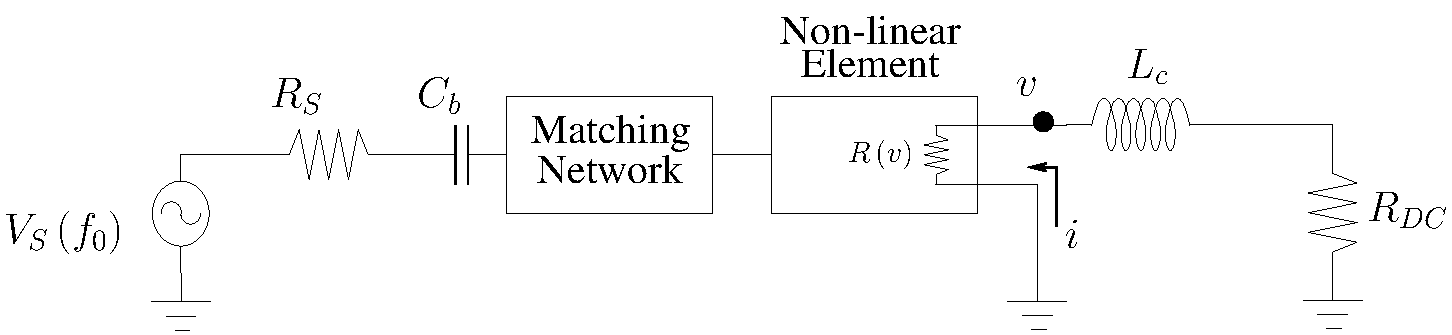
\includegraphics[width=3.5in]{pdf/01.pdf}\\
  \caption{score and number of reviews ratio}\label{score_reviews_ratio}
  \end{center}
\end{figure}


The conversion efficiency, defined as the ratio of the DC power dissipated in the load resistor to the available fundamental frequency RF power, is evaluated as


Therefore, the ideal half-wave rectifier converts all available RF power to DC power if the the DC loading resistance set to the value given in (\ref{DC_resistance}). The RF-DC conversion efficiency as a function of $R_{DC} / R_s(f_0)$ was simulated in Microwave Office$\textsuperscript{\textregistered}$ for varying rectifier on-resistance and is shown in Fig.~\ref{sim_opt_eff_classFinv}. The harmonic balance settings were identical to those used for the class-C rectifier above. The peak efficiency as a function of on-resistance is higher than for the class-C rectifier, although the efficiency degrades more quickly when the non-ideal DC load is applied.

%For zero on-resistance, the optimal DC load is exactly that predicted by (\ref{DC_resistance}).
%The reason for the increase in optimal DC load as the on-resistance increases is that the current
%through the on-resistance is reduced, thus reducing the loss.  However, there is a penalty paid in
%reflected power from the rectifying element due to the non-ideal match.  This limits the benefit of
%increasing the DC load infinitely with a fixed fundamental frequency match.  Theoretically, if the
%fundamental and DC loads could be increased infinitely the efficiency would approach 100\,\% no matter
%how large the on-resistance became.
%
% SHOULD WE MAYBE MOVE THIS TO DISCUSSION OR POSSIBLY DELETE?

% ==== FIG 4
\begin{figure}[!b]
  \begin{center}
  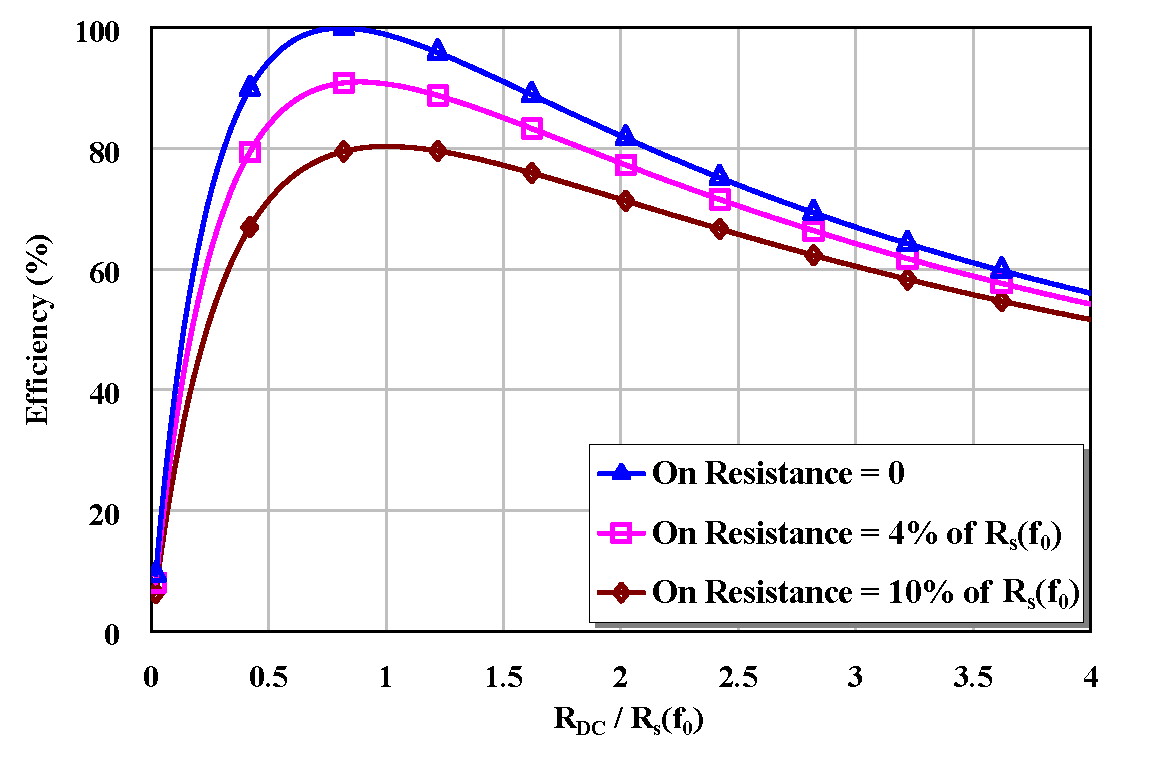
\includegraphics[width=3.5in]{pdf/04.pdf}
  %  \vspace{-15pt}
  \caption{Simulated efficiency of class-F$^{-1}$ rectifier versus $R_{DC} / R_s(f_0)$ for varying rectifier on-resistance.}\label{sim_opt_eff_classFinv}
  \end{center}
\end{figure}

The waveforms including parasitic on-resistance and threshold voltage are next investigated assuming the rectifier impedance from (\ref{nonideal_rectifier_resistance}). The time domain voltage and current waveforms are approximated as
\begin{equation}\label{diode_voltage_waveform_finv_par}
v(\theta) =
\begin{cases}
    V_{max}\sin\theta, & v(\theta) > -V_{tr}\\
    -V_{tr} - I_{max}R_{on}, & v(\theta) \leq -V_{tr}
\end{cases}
\end{equation}
\begin{equation}\label{diode_current_waveform_finv_par}
i(\theta) =
\begin{cases}
    0, & V(\theta) > -V_{tr}\\
    I_{max}, & v(\theta) \leq -V_{tr}
\end{cases}
\end{equation}



% === FIG 5
\begin{figure}[!b]
  \begin{center}
  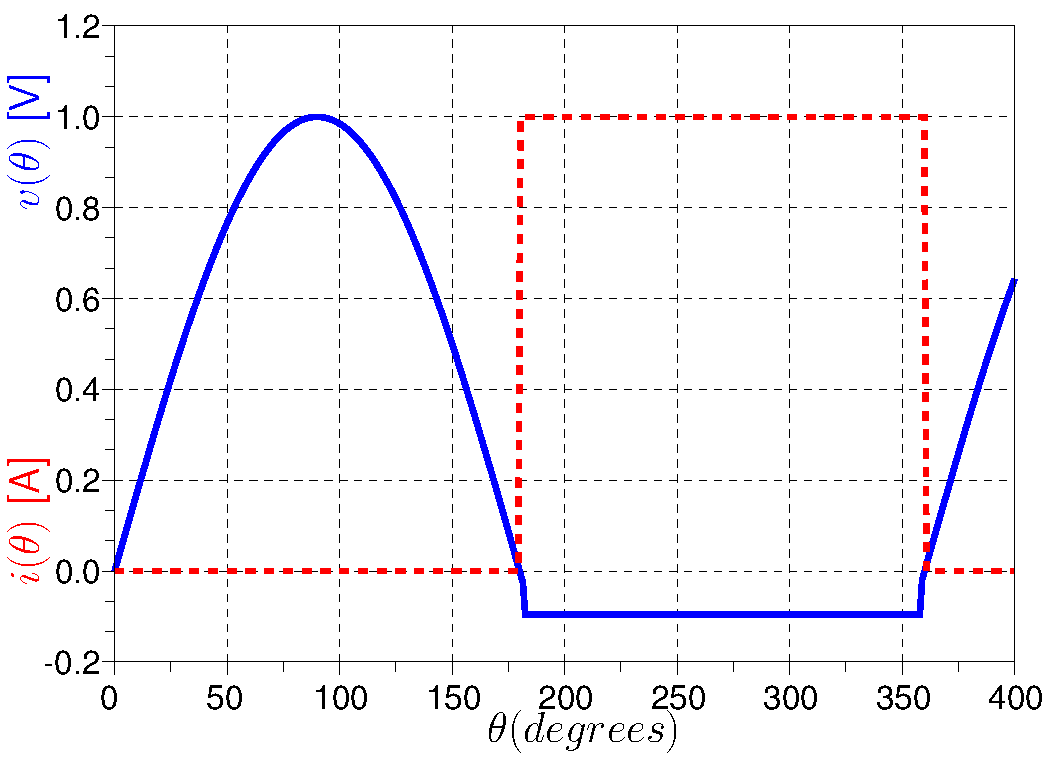
\includegraphics[width=3.0in]{pdf/05.pdf}
     % \vspace{-5pt}
  \caption{\hl{Non-ideal class-F$^{-1}$ voltage (solid) and current (dashed) waveforms, normalized to their peak respective values.}}\label{finv_waveform_nonideal}
  \end{center}
\end{figure}

As an example, Fig.~\ref{finv_waveform_nonideal} shows the current and voltage waveforms for a specific set of non-ideal parameters ($V_{tr} = 0.7\,\textrm{V}$, $V_{max} = 20\,\textrm{V}$, $I_{max} = 200\,\textrm{mA}$, and $R_{on} = 5\,\Omega$). When the device is conducting current, it creates a voltage drop across the on-resistance which is constant due to the constant current. If the on-resistance were zero, the only difference between the waveform in (\ref{diode_voltage_waveform_finv_par}) and the ideal voltage waveform would be the minimum value, which would be $-V_{tr}$ rather than zero. The values of $\theta$ at which the transition between the conducting and non-conducting regions occurs are found to be
\begin{equation}\label{trans_points_thetafinv2}
\begin{array}{l}
    \theta_{t1} = 2\pi - \arcsin\left(\frac{V_{tr}}{V_{max}}\right) \\
    \theta_{t2} = \pi + \arcsin\left(\frac{V_{tr}}{V_{max}}\right)
\end{array}
\end{equation}

The DC and fundamental frequency values of the voltage and current waveforms can be found through a Fourier analysis using the transition points in (\ref{trans_points_thetafinv2}). The first Fourier coefficient of $v(t)$ gives the DC component of the voltage, which can be derived as
\begin{equation}\label{finv_dc_comp_5}\begin{split}
    V_{DC} &= \frac{1}{2\pi}\left(2V_{max}\sqrt{1 - \left(\frac{V_{tr}}{V_{max}}\right)^2} \right. \\
    &-(V_{tr} + I_{max}R_{on})\left[\pi - 2\arcsin\left(\frac{V_{tr}}{V_{max}}\right)\right]\Bigg)
\end{split}\end{equation}

The fundamental frequency voltage is found from $V(f_0)=a_v+jb_v$, where
\begin{shaded}
\begin{equation}
a_v=\frac{1}{\pi}\int_0^{2\pi}v(\theta)\cos \theta d\theta = 0
\end{equation}
\end{shaded}
and $b_v$ can be reduced to


\begin{equation}\label{finv_vf0_comp_5}\begin{split}
    b_v =& \frac{1}{\pi}\Bigg(V_{max}\arcsin\left(\frac{V_{tr}}{V_{max}}\right)+ \frac{\pi V_{max}}{2}  \\
    &+ \left.\left(V_{tr} + 2I_{max}R_{on}\right) \sqrt{1 - \left(\frac{V_{tr}}{V_{max}}\right)^2}\right)
\end{split}\end{equation}

Similarly, the DC component of the current waveform is found to be

\begin{equation}\label{finv_idc_comp_3}
    I_{DC} = \frac{I_{max}}{2\pi}\left(\pi - 2\arcsin\left(\frac{V_{tr}}{V_{max}}\right)\right)
\end{equation}
The fundamental frequency current $i(t)=a_i+jb_i$ has $a_i=0$ and the coefficient $b_i$ can be shown to be equal to

\begin{equation}\label{finv_if0_comp_2}
    b_i = -\frac{2I_{max}}{\pi}\sqrt{1 - \left(\frac{V_{tr}}{V_{max}}\right)^2}
\end{equation}
The input power \hl{at the fundamental frequency} is found from 


\begin{equation}\label{Pin}
  P_{in} = \Re\left\{\frac{V(f_0)I^{*}(f_0)}{2}\right\}
\end{equation}


\hl{Substituting (}\ref{finv_vf0_comp_5}) and (\ref{finv_if0_comp_2}) into the above results in

\begin{shaded}
\begin{equation}\begin{split}\label{Pin_diode2}
    P_{in} =& \frac{kI_{max}}{\pi^2}\left(V_{max}\arcsin\left(\frac{V_{tr}}{V_{max}}\right) + \frac{\pi V_{max}}{2} \right. \\
   &+ \left(V_{tr}+2I_{max}R_{on}\right)k\bigg)
\end{split}\end{equation}
\end{shaded}
where $k$ is defined as
\begin{equation}\label{k}
    k = \sqrt{1 - \left(\frac{V_{tr}}{V_{max}}\right)^2}
\end{equation}

Solving for $I_{max}$ as a function of $P_{in}$ when $R_{on}$ is non-zero after some arithmetic results in two solutions, one of which is negative. The positive solution for the maximal current is

\begin{equation}\label{Imax_solved1}
    I_{max} = \frac{ \sqrt{\alpha^2 + 8\pi^2P_{in}R_{on}}-\alpha}{4R_{on}k}
\end{equation}
with $\alpha=V_{max}\left(\arcsin\left(\frac{V_{tr}}{V_{max}}\right)+ \frac{\pi}{2} + k\frac{V_{tr}}{V_{max}}\right)$.

In the case where $R_{on}$ is zero, (\ref{Imax_solved1}) simplifies to
\begin{equation}\label{Imax_solve_zeroron_solved}
    I_{max} = P_{in}\frac{\pi^2}{kV_{max}\left(\arcsin\left(\frac{V_{tr}}{V_{max}}\right)+ \frac{\pi}{2} + k\frac{V_{tr}}{V_{max}}\right)}
\end{equation}

Note that in the case of an ideal rectifying element, $k = 1$ and $V_{tr} = 0$, therefore
\begin{equation}\label{Imax_solve_zeroron_solved_ideal}
    I_{max,ideal} = \frac{2\pi P_{in}}{V_{max}}
\end{equation}

Now that $I_{max}$ is fully expressed given known rectifier parameters, $V_{DC}$ and $I_{DC}$, $V(f_0)$ and $I(f_0)$ may be calculated, and from this, the DC load and the load at fundamental frequency determined from the following expressions:

\begin{equation}\label{rdcf}
    R_{DC} = \frac{V_{DC}}{I_{DC}}
\end{equation}

\begin{equation}\label{rf0f}
    R(f_0) = -\frac{V(f_0)}{I(f_0)} = -\frac{b_v}{b_i}
\end{equation}
The negative impedance in (\ref{rf0f}) indicates that power is delivered to the rectifying element and gives the impedance of the source delivering power to the rectifying element.  The rectifier efficiency is given by
\begin{equation}\label{efff}
    \eta = \frac{P_{DC}}{P_{in}} = \frac{V_{DC}I_{DC}}{P_{in}}
\end{equation}










\subsection {Design example based on class-F$^{-1}$ theory}

To understand the usefulness of the presented theory, assume the rectifying element has the following parameters: $V_{max} = 10$\,V, $R_{on} = 5$\,$\Omega$, $V_{tr} = 0.7$\,V and $P(f_0)$ = 1\,W.  First, (\ref{Imax_solved1}) is used to calculate $I_{max}=456.7$\,mA. Next, the DC voltage and current are evaluated using (\ref{finv_dc_comp_5}) and (\ref{finv_idc_comp_3}), respectively, to give $V_{DC}=1.75$\,V and $I_{DC}=218.2$\,mA. The fundamental frequency voltage and current Fourier coefficients are then calculated to be $V(f_0)=6.896$\,V and $I(f_0)=-290$\,mA, respectively.  The DC and fundamental frequency resistances are then calculated using (\ref{rdcf}) and (\ref{rf0f}) to be $R_{DC}=8.02$\,$\Omega$ and $R(f_0)=23.77$\,$\Omega$, respectively.  The efficiency is then calculated using (\ref{efff}) to be $\eta$ = 38.18\,\%. If the input power is selected as 0.1\,W rather than 1\,W, the resultant efficiency is 72.43\,\% instead.  A specific rectification device will always have an approximate input drive level at which it can be most efficient, just as with power transistors in power amplifiers. To maximize efficiency, the goal is always to minimize the amount of power dissipation in the on-resistance of the rectifying element and maximize the power dissipated in the DC load resistor.









% === III. Schottky-Diode Class-C Rectifier =======================================
% =================================================================================
\section{Schottky-Diode Class-C Rectifier}

The Skyworks SMS7630 Schottky diode in the SC-79 package was selected for the half-wave rectifier. Source-pull was performed at 2.45\,GHz with 0-10\,dBm available input power for various DC loads in order to identify the combination of input power, fundamental load and DC load resulting in highest efficiency.  The best case occurred at 6\,dBm input power, with the source-pull contours being shown in Fig.~\ref{lpcontours}.  The on-resistance of the SMS7630 is 20\,$\Omega$ with the optimal DC load of 1080\,$\Omega$. Therefore $R_{on}$ is approximately 2\% of $R_{DC}$\hl{,} which in theory is 4\% of $R_s(f_0)$.  From Fig.~\ref{sim_opt_eff}, a peak efficiency of 87\% occurs with infinite harmonic terminations, therefore the achieved 77.6\% is very reasonable considering only the 2$^{\rm nd}$ and 3$^{\rm rd}$ harmonics were explicitly terminated.



\begin{figure}
  \begin{center}
  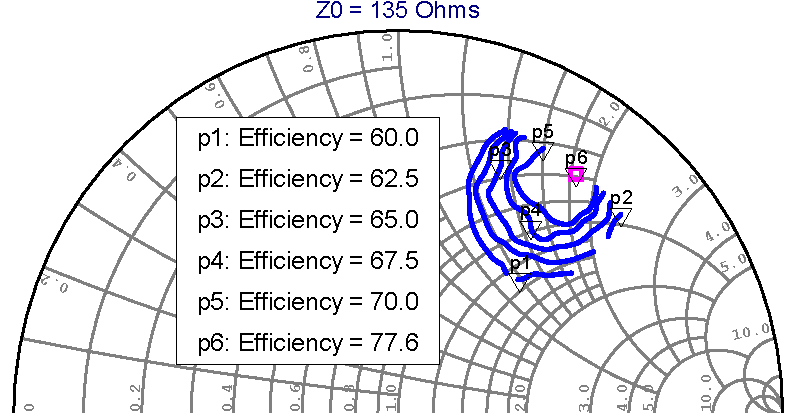
\includegraphics[width=3.0in]{pdf/06.pdf}\\
 \caption{\hl{Source-pull contours with available input power to the diode set to 6\,dBm.  The impedance is referenced to the junction capacitance of the diode, therefore the lead inductance of the package has been compensated for. Setting $R_{DC}$ to 1080\,$\Omega$ was found to result in the optimal efficiency for this input power. The highest efficiency of 77.6\% is obtained at $Z_{p6}=(68+j245)\Omega$ with $V_{DC}$=1.82\,V.}}\label{lpcontours}
  \end{center}
\end{figure}
 
%  \caption{Source-pull contours with available input power to the diode set to 6\,dBm.  The impedance is referenced to the junction capacitance of the diode, therefore the lead inductance of the package has been compensated for. Setting $R_{DC}$ to 1080\,$\Omega$ was found to result in the optimal efficiency for this input power.}\label{lpcontours}


\begin{figure}
  \begin{center}
  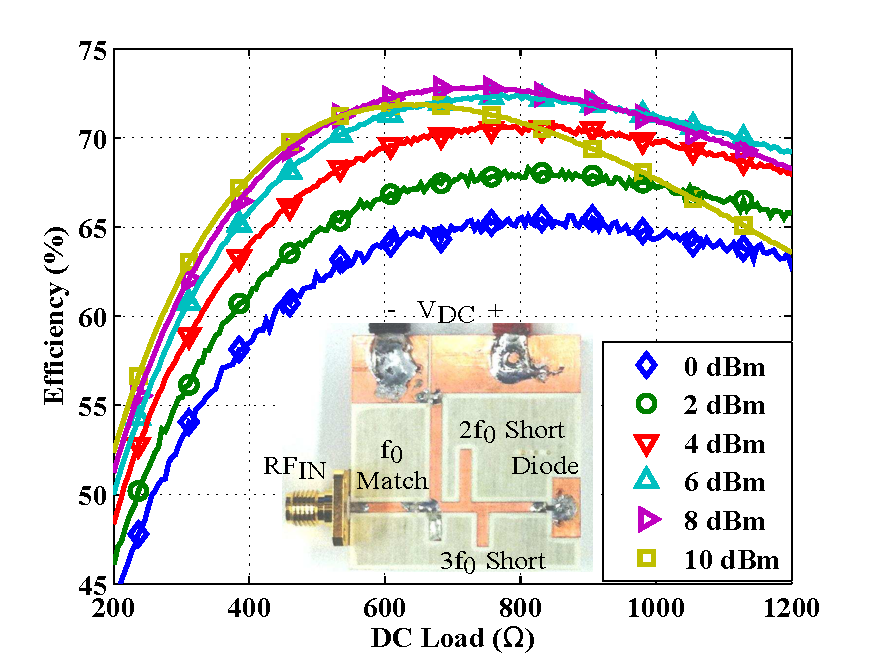
\includegraphics[width=3.5in]{pdf/07.pdf}\\
 \caption{\hl{RF-DC conversion efficiency versus DC load for fixed available input powers with 0.6\,dB matching network loss de-embedded.  The maximum efficiency of 72.8\% occurred at 8\,dBm with $R_{DC}$ = 742\,$\Omega$ and $V_{DC}$=1.91\,V, which is lower than the 1080\,$\Omega$ found during source-pull.  However, the efficiency at 1080\,$\Omega$ is 69.9\% which is very close to the peak value.}}\label{final_dc_sweep}
  \end{center}
\end{figure}
 
%  \caption{RF-DC conversion efficiency versus DC load fixed available input powers with 0.6\,dB matching network loss de-embedded.  The maximum efficiency of 72.8\% occurred at 8\,dBm with $R_{DC}$ = 742\,$\Omega$, which is lower than the 1080\,$\Omega$ found during source-pull.  However, the efficiency at 1080\,$\Omega$ is 69.9\% which is very close to the peak value.}\label{final_dc_sweep}


Measurements of a rectifier designed using the source-pull data show a maximum RF-DC conversion efficiency of 72.8\% when matched to 50$\Omega$, obtained after the 0.6\,dB matching network loss is de-embedded.  The fabricated rectifier and DC load sweep measurements are shown in Fig.~\ref{final_dc_sweep}. Open circuit shunt stubs are used to present short-circuit terminations at the second and third harmonic.  A shunt capacitor is used for presenting the fundamental frequency impedance to reduce size and allow tunability.  The reduction in efficiency relative to the source-pull measurements is due to the matching circuit not presenting the ideal impedance found during source-pull.





The class-C rectifier can be applied to improving the efficiency of a wireless powering reception device as demonstrated in \cite{robergIMS2012} with a dual-linearly polarized patch rectenna, with a rectifier circuit for each polarization. In this circuit, the first 5 harmonics are shorted and the impedances are validated by calibrated measurements and are presented in \cite{robergIMS2012}.















% === IV. Transistor Class-F inv Rectifier ========================================
% =================================================================================
\section{Transistor Class-F$^{-1}$ Rectifier}

To prove experimentally the duality between harmonically terminated PAs and rectifiers, a high-efficiency class-F$^{\rm -1}$ PA was designed, measured first as an amplifier, and then as a rectifier. In the rectifier measurements, RF power is input into the drain which is unbiased. The gate is terminated in a variable impedance and biased close to pinch-off. Measurements of efficiency and DC voltage are performed in time domain as a function of input RF power, gate RF load, gate bias and drain DC load. 

\subsection {Circuit design}

A 2.14-GHz power amplifier, pictured on Fig.~\ref{amplifier}, is designed using the Triquint TGF2023-02 GaN pHEMT \cite{gan_pa_letter}. Class F$^{-1}$ harmonic terminations are implemented at the second and third harmonic. The performance of the PA, illustrated in  Fig.~\ref{PA_meas}, was characterized at 2.14\,GHz with a drain voltage bias of 28\,V and a bias current of 160\,mA. The PA exhibits a PAE of 84\% with an output power of 37.6\,dBm and a gain of 15.7\,dB under 3\,dB compression. The same PA design was used for rectifier measurements as shown in Fig.~\ref{measurement_setup}. \hl{The PA is connected to an input RF source at the drain, with the drain supply disconnected. The gate terminal is biased, and connected to an impedance tuner, converting the two-port transistor PA to a one-port rectifier, corresponding to the generalized schematic of Fig.}~\ref{circuit_diagram}.

% === FIG : Amplifier Picture
\begin{figure}[ht!]
\centering
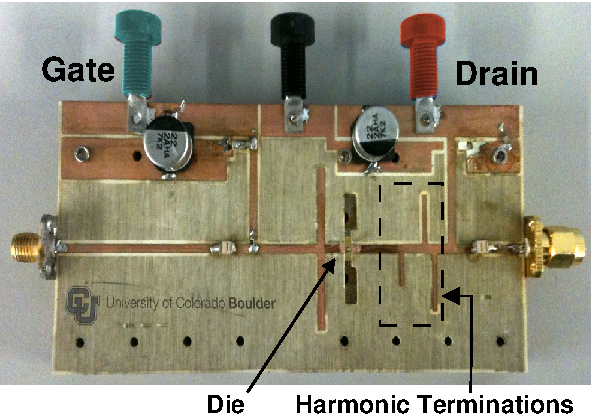
\includegraphics[width=3.0in]{pdf/08.pdf}
\caption{Photograph of the class-F$^{-1}$ power amplifier, working at 2.14 GHz and presented in \cite{gan_pa_letter}.}
\label{amplifier}
\end{figure}


% === FIG : PA measurements
\begin{figure}
  \begin{center}
  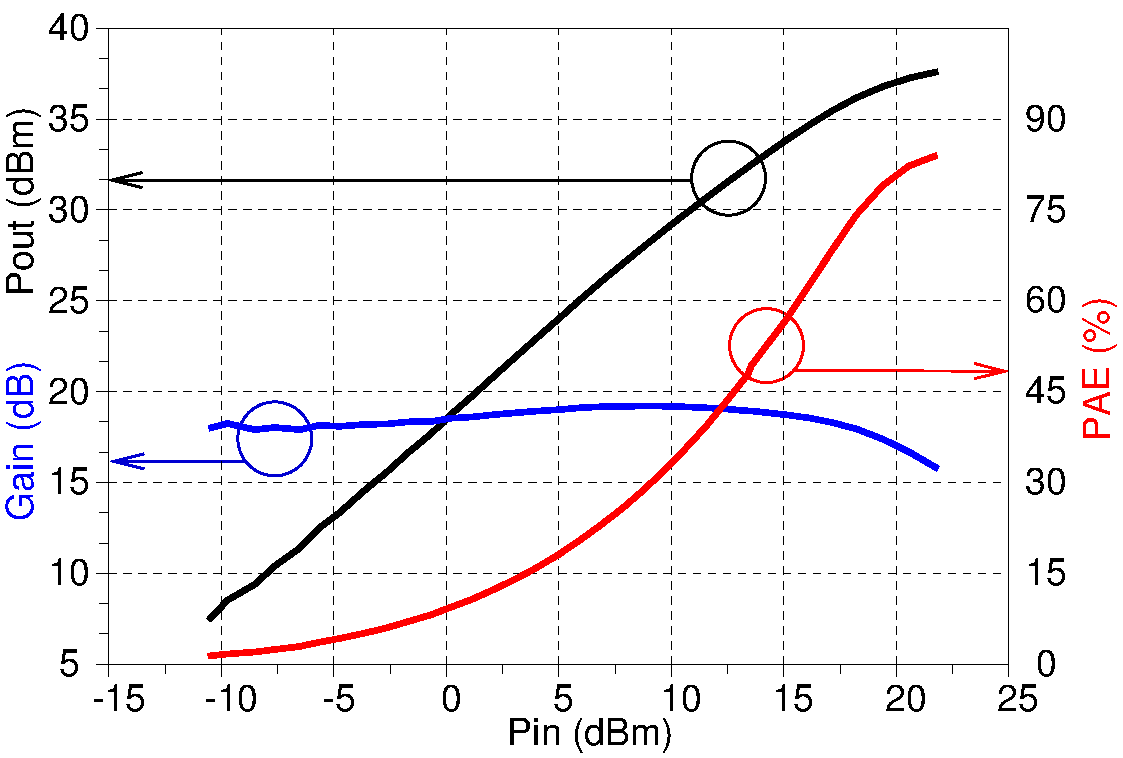
\includegraphics[width=3.0in]{pdf/09.pdf}
  \caption{\hl{Large-signal measurements performed on the class-F$^{-1}$ power amplifier at $f_0=2.14$\,GHz, $V_{GS}=-3.8$\,V and $V_{DS}=28$\,V}}
\label{PA_meas}
  \end{center}
\end{figure}









\subsection {Measurement setup}
% 
The class-F$^{\rm -1}$ power amplifier described above is fully characterized in large signal in a rectifier configuration with the setup shown in Fig.~\ref{measurement_setup}. The commercial time-domain large signal measurement instrument is a VTD SWAP four-channel receiver \cite{SWAP}. In order to acquire time domain waveforms at the reference plane, an 8 error term model calibration similar to the one performed for LSNA \hl{(Large Signal Network Analyzer)} measurements is applied. After \hl{an absolute VNA-like calibration} \cite{verspecht}, the RF voltage and current waveforms at the input (V1 and I1) and at the output (V2 and I2) of the DUT are measured at the coaxial reference plane. In this case, the RF input is the drain port of the PA, while the RF output is connected to the gate port. Thus, performing a load pull on this device consists of varying the load at $f_0$ at the RF gate port of the PA with a passive tuner. This kind of measurement is similar to large signal characterization of switch devices recently reported in \cite{switch,faraj_arftg_2012}. The gate DC path is connected to a power supply so the gate bias can be varied. The drain DC bias is the output of the rectifier and is connected to a variable resistance $R_{DC}$, and the DC voltage across it is measured with a voltmeter. The DC current is then found from the value of $R_{DC}$ from (\ref{rdcf}). During the measurement, several parameters are varied systematically: the RF load impedance applied at the PA gate port $Z_g(f_0)=V_g(f_0)/I_g(f_0)$; the resistor in the DC drain output $R_{DC}$; and the gate bias voltage $V_{GS}$. The conversion efficiency of the rectifier and the DC power delivered at the drain output of the rectifier $P_{DC}= V_{DC} \cdot I_{DC}$ are measured as these parameters are varied, and as a function of input power at the drain port $P_{in}(f_0)$.





\begin{figure}[ht!]
\centering
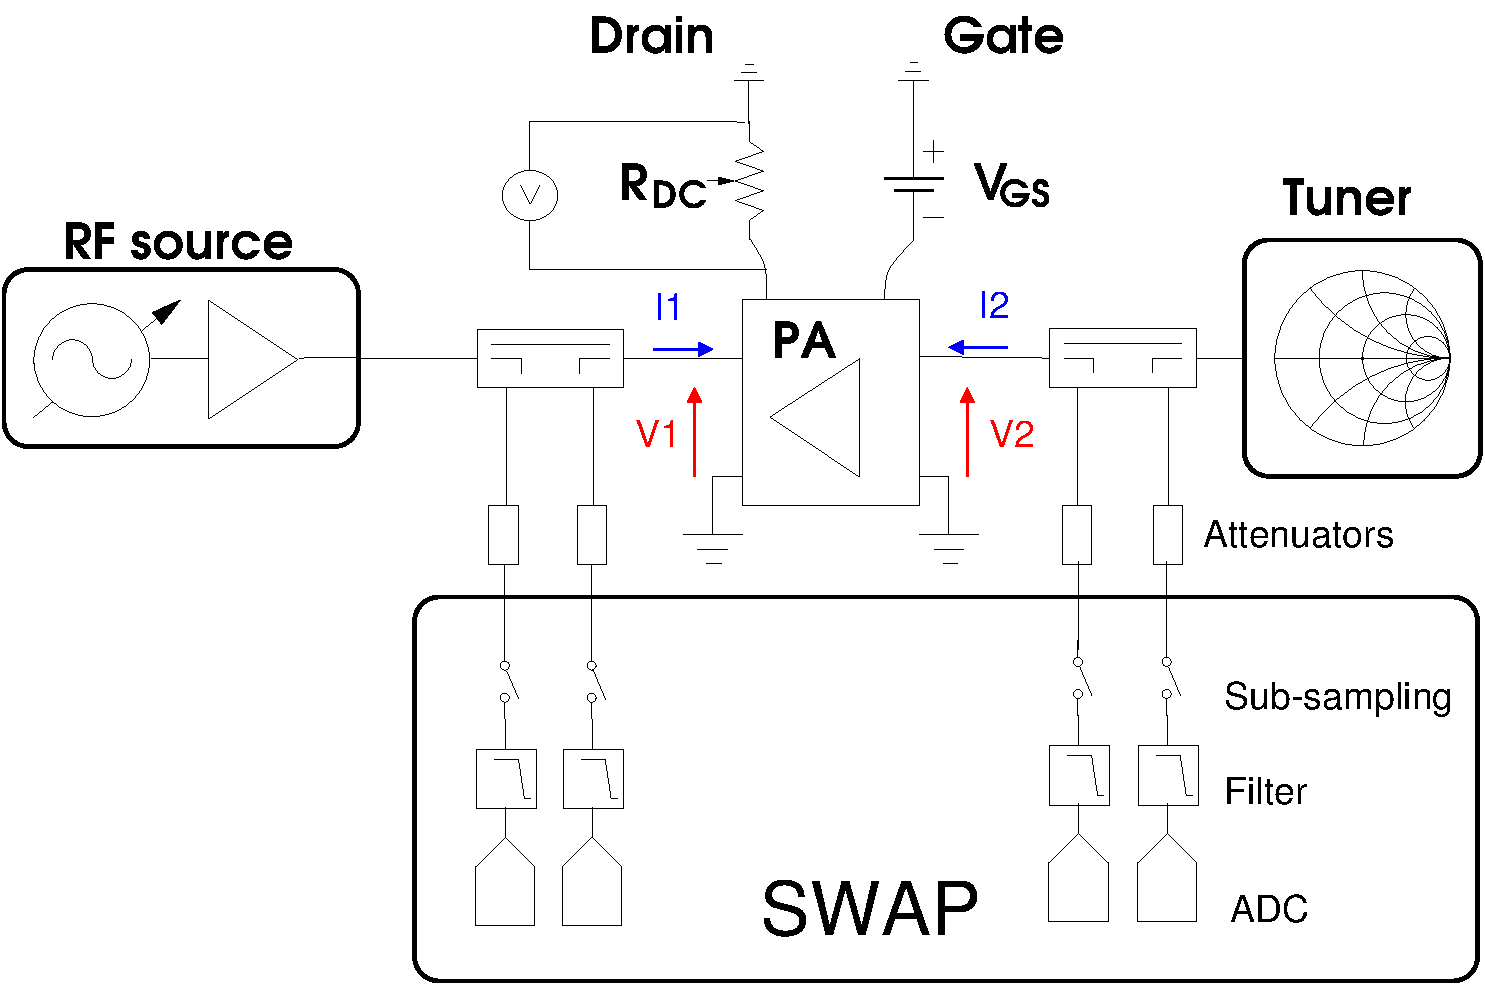
\includegraphics[width=3.5in]{pdf/10.pdf}
\caption{Time-domain non-linear rectifier measurement block diagram. The SWAP \cite{SWAP} performs sampling of current and voltage and the calibration refers the sampled quantities to the reference planes at the DUT. The drain output DC resistance $R_{DC}$ , the gate bias $V_{GS}$ and the gate RF impedance $Z_g$ are varied as the input power at the drain is swept from 10 to 42\,dBm.}
\label{measurement_setup}
\end{figure}














\subsection {Self-synchronous transistor rectifier results}

The measurements of the rectifier are performed in self-synchronous mode, i.e. there is no input RF power incident externally into the gate port of the PA, unlike in previous transistor rectifier work \cite{JoseIMS-rect,Kaz}. The following parameters are varied in order, while keeping the other parameters constant and sweeping the input RF power at the drain port, and the results are described in the same order:

\begin{enumerate}
\item RF impedance at the gate, $Z_g$;
\item load resistance at drain bias output, $R_{DC}$;
\item gate DC bias, $V_{GS}$.
\end{enumerate}

%\subsubsection{Sweeping \textbf{Tuner} - the RF load impedance at $f_0$ at the output (gate access)}
The gate load-pull was performed to determine the optimum impedance for maximum efficiency with a constant resistive DC load of 98.5\,$\Omega$ (nominally 100\,$\Omega$) and a constant transistor gate bias in pinch-off of -4.4\,V. The RF signal is coupled from the drain to the gate matching network through the feedback capacitance $C_{gd}$, and thus the precise impedance presented at the gate of the transistor is imperative to achieving high efficiency. Fig.~\ref{time-domain} shows the time-domain voltage and current waveforms measured at the drain and gate RF port of the amplifier when the RF input power at the drain port is swept from 11\,dBm to 42\,dBm. These values are chosen because the rectifier in PA operation gives up to 42\,dBm output power. The feedback signal present at the gate allows for the rectifier to operate in self-synchronous mode without any additional control signal. Unlike in the synchronously driven case where an external generator is connected to the gate, here the impedance presented at the gate is always passive (inside the Smith chart), keeping the device in a safe operating mode.

% === FIG : Time-domain waveforms
\begin{figure}[ht!]
\centering
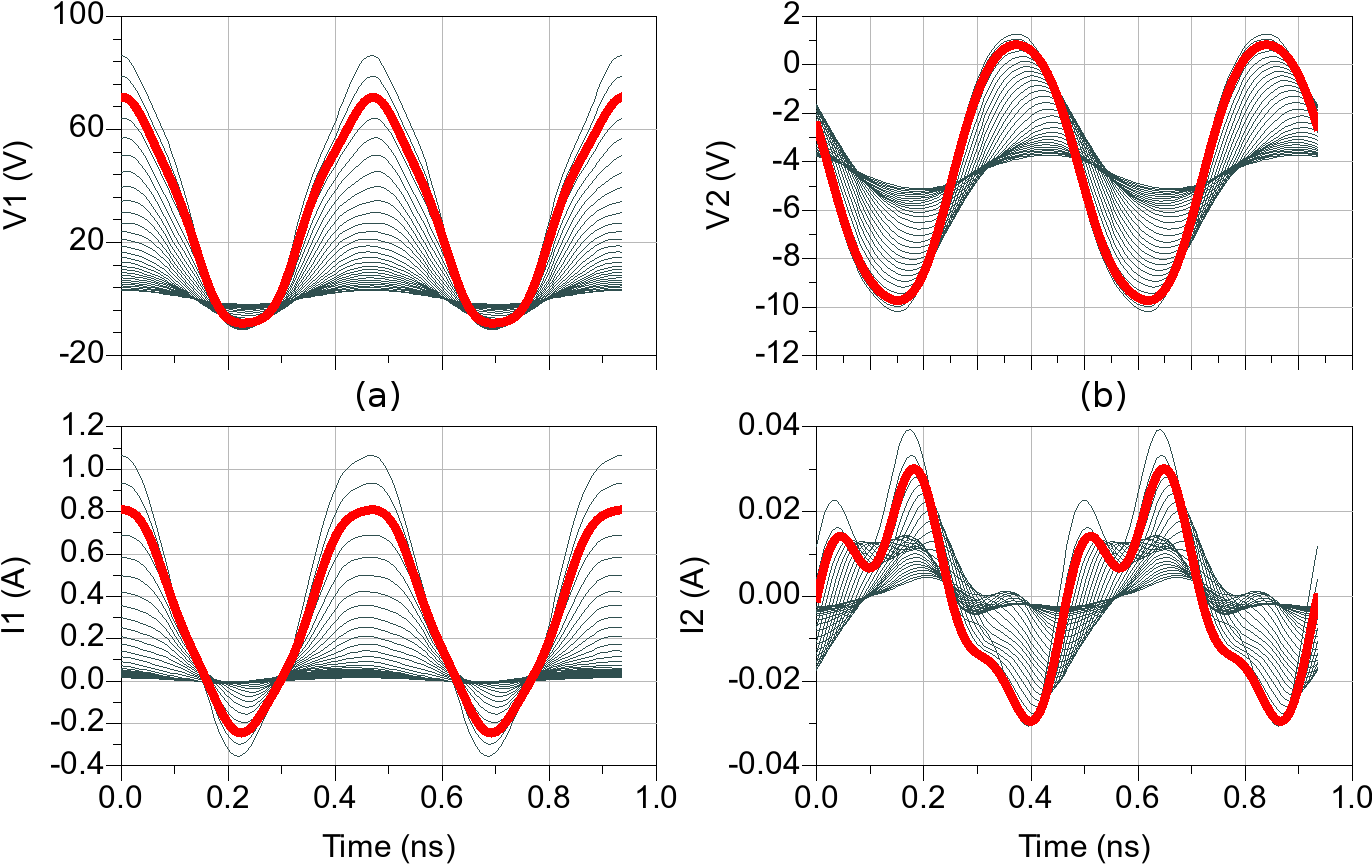
\includegraphics[width=3.4in]{pdf/11.png}
\caption{\hl{Time-domain waveforms measured at drain (a) and gate (b) of the rectifier with $V_{GS}=-4.4$\,V, $R_{DC}=98.5$\,$\Omega$ and $Z_g(f_0)=\left(230+j10\right)\Omega$. The RF input power at the drain is swept from 10 to 42\,dBm, corresponding to the range of output power of the class-F$^{-1}$ PA.}}
\label{time-domain}
\end{figure}

Measured RF-DC conversion efficiency is shown in Fig.~\ref{MEAS_LP_sweep} for four different RF gate impedances. A maximal conversion efficiency of 85\% is achieved with a DC output voltage of 36\,V and an input power at the drain of 42\,dBm \hl{with $R_{DC}=98.5\,\Omega$}. This peak efficiency is for a RF gate load of around 230\,$\Omega$ (green \hl{hexagon} in the Smith chart in Fig.~\ref{MEAS_LP_sweep}), which is the highest impedance that was achievable with the specific tuner in the setup. For the low gate impedance (red \hl{triangle} in the Smith chart), the efficiency is significantly lower. By observing the gate current (Fig.~\ref{MEAS_LP_sweep}d), it can be seen that for a low RF gate impedance, the gate diode turns on at around $P_{in}=25$\,dBm. Since the input power cannot be increased much beyond this point to avoid breakdown, this limits the DC voltage at the output to around 4\,V. For the gate impedance with highest efficiency (\hl{green line with hexagon symbol}), the gate diode is off for input drain powers below 41\,dBm, allowing for high DC voltage output.


%talk about Gate Idc ?




% === FIG : LP SWEEP
\begin{figure}[ht!]
\centering
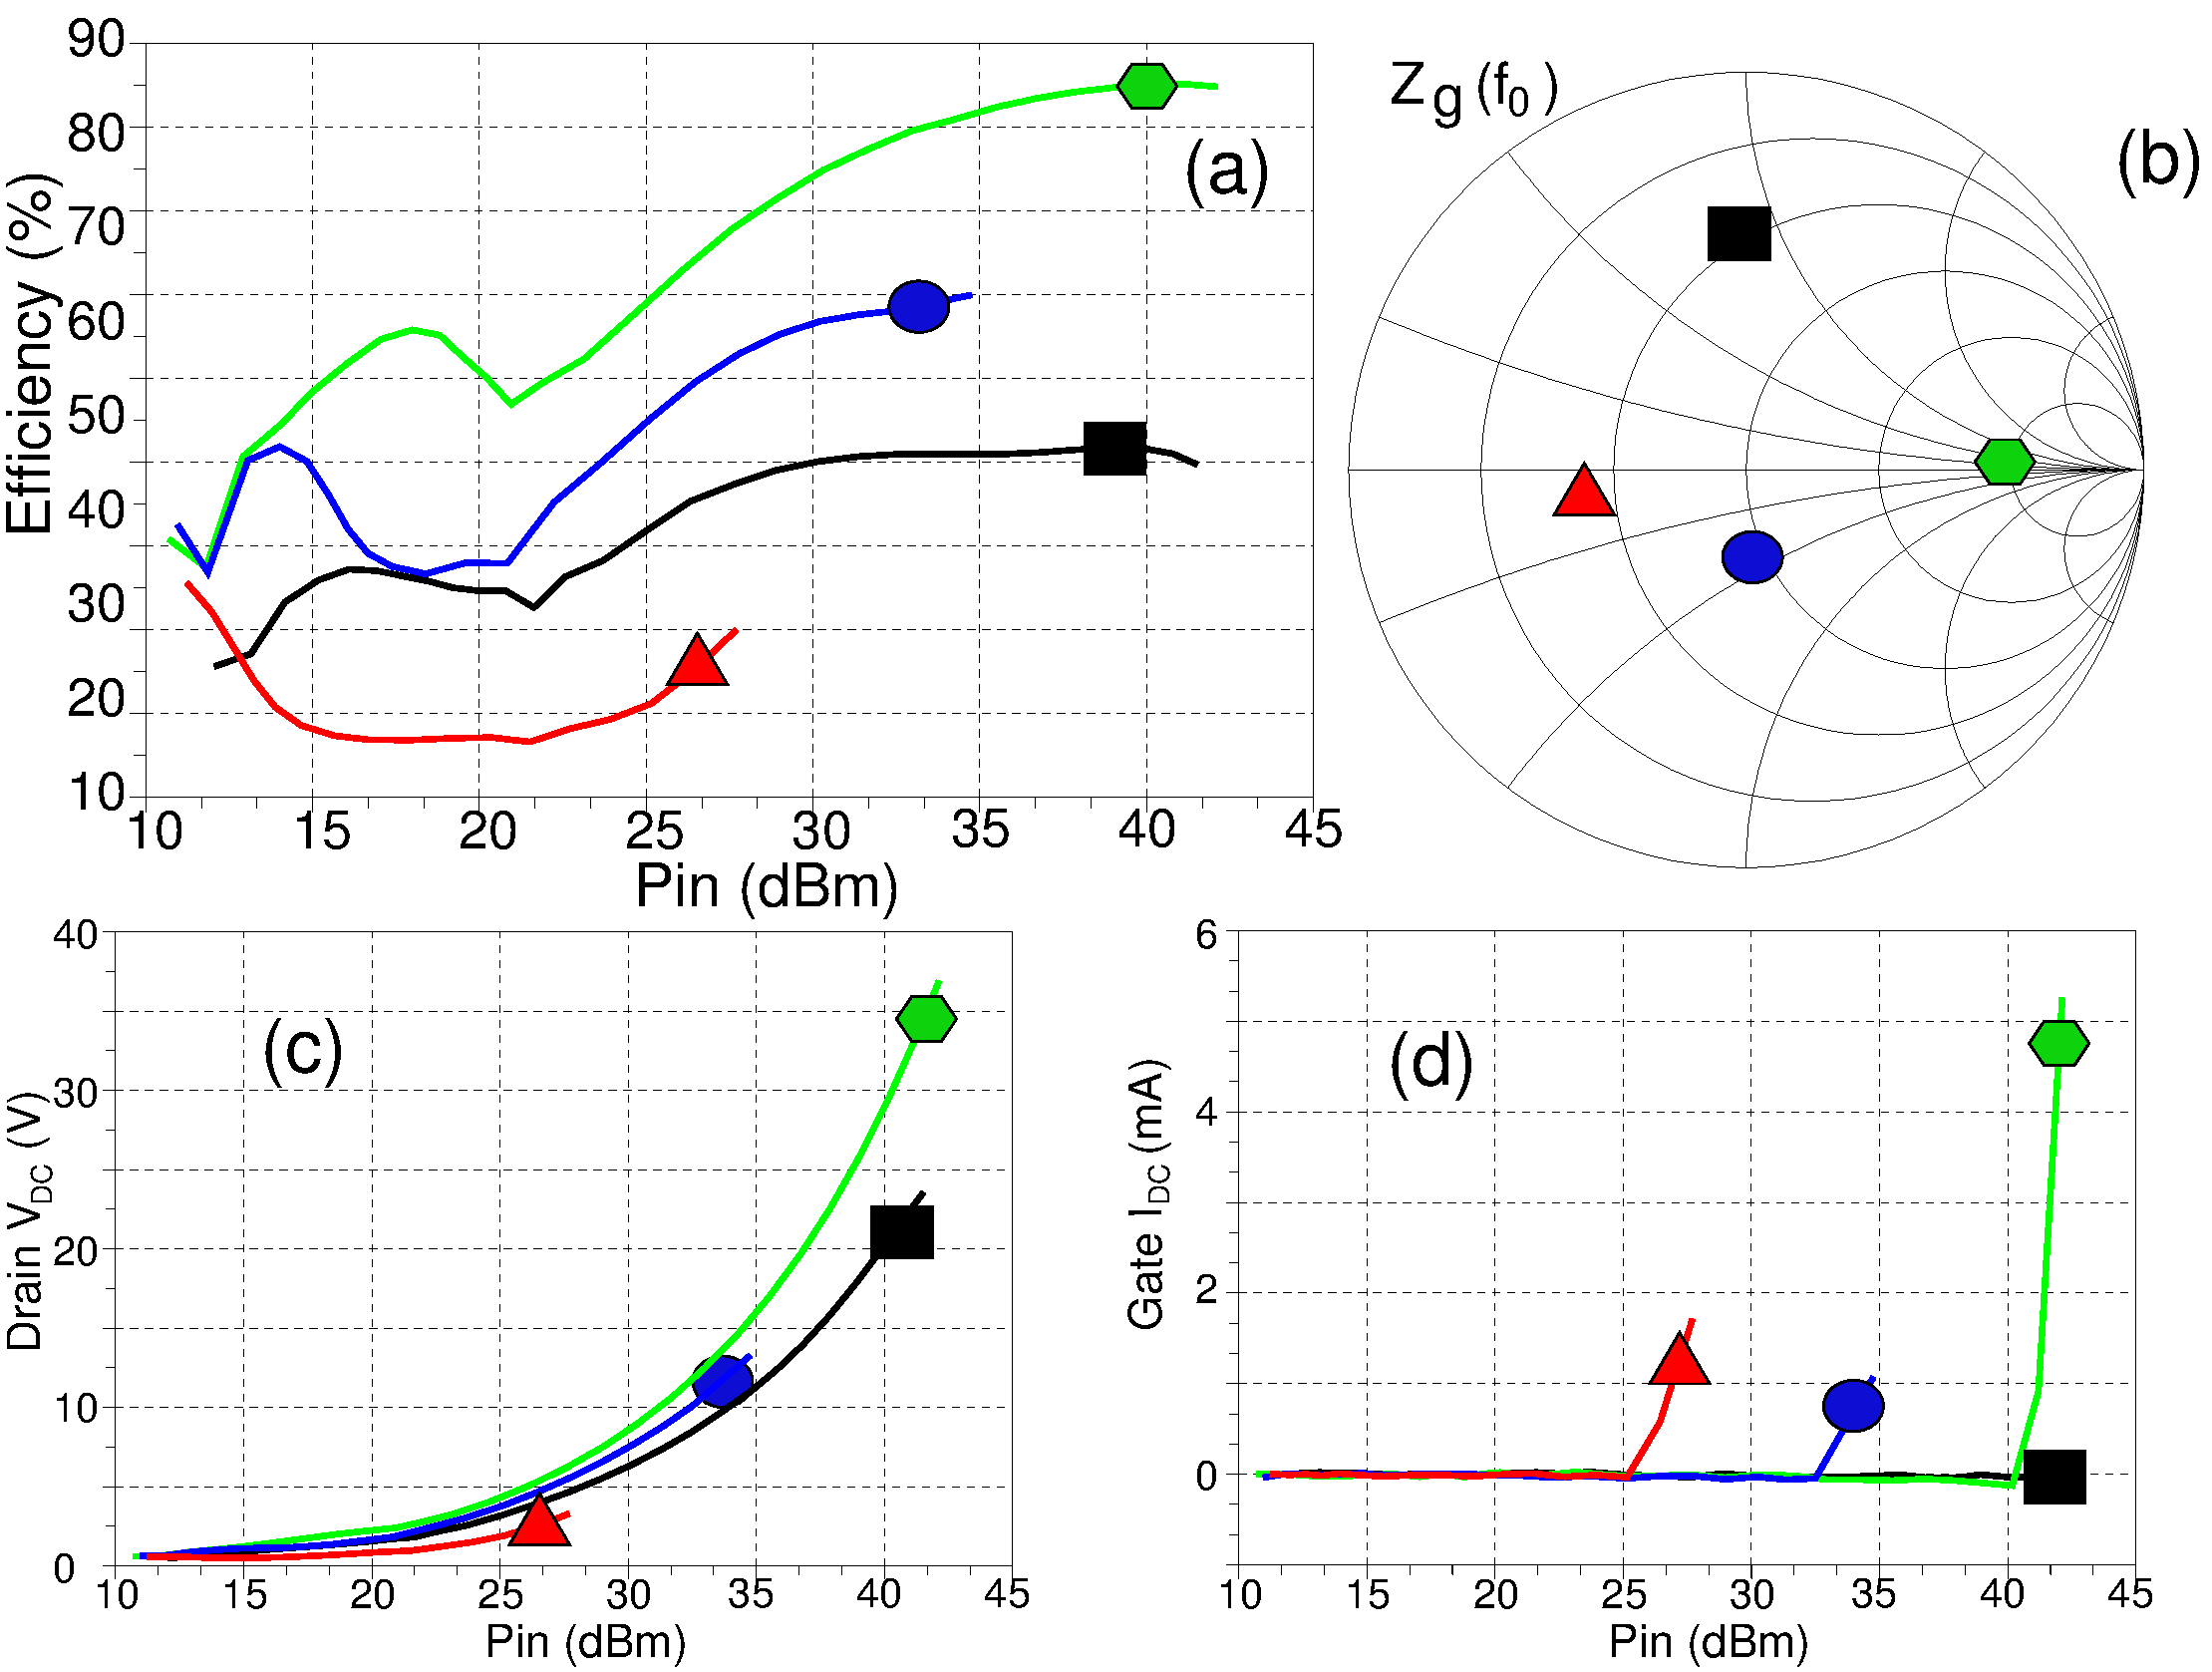
\includegraphics[width=3.4in]{pdf/12.pdf}
\caption{\hl{Conversion efficiency, gate DC current and drain DC voltage versus input power for several RF load impedance values presented at the gate. $V_{GS}=-4.4$\,V and $R_{DC}=98.5$\,$\Omega$. The green point on the Smith chart corresponds to the highest efficiency point at $Z_g(f_0)=\left(230+j10\right)\Omega$. }}
\label{MEAS_LP_sweep}
\end{figure}





% ===================================================================================================================================
% ===================================================================================================================================


%\subsubsection{Sweeping \textbf{Rd} - the resistance at the DC drain access}
After the optimal gate impedance for highest efficiency was obtained, a power sweep for three different $R_{DC}$ values in the drain output was obtained. From Fig.~\ref{Rd_sweep_final}, a maximal efficiency of 85\% was measured for a DC resistive load of 98\,$\Omega$ while an efficiency drop of 13\% was observed for a DC load of 21\,$\Omega$ with 40\,dBm input power. As expected, the DC output voltage decreases from a maximum \hl{30\,V} for $R_{DC}=98$\,$\Omega$ at 40\,dBm input power, to a maximum of 13.4\,V for $R_{DC}=21$\,$\Omega$ with the same input power. It is interesting to see how the input impedance of the rectifier at the RF drain port approaches 50\,$\Omega$ as the input power increases, Fig.~\ref{Rd_sweep_Zin}. This is expected, since the PA was designed for maximal saturated power delivered into a 50\,$\Omega$ load. This again points to the similarities between the same circuit operated as a power rectifier and a power amplifier.

% === FIG : Rd SWEEP
\begin{figure}[ht!]
\centering
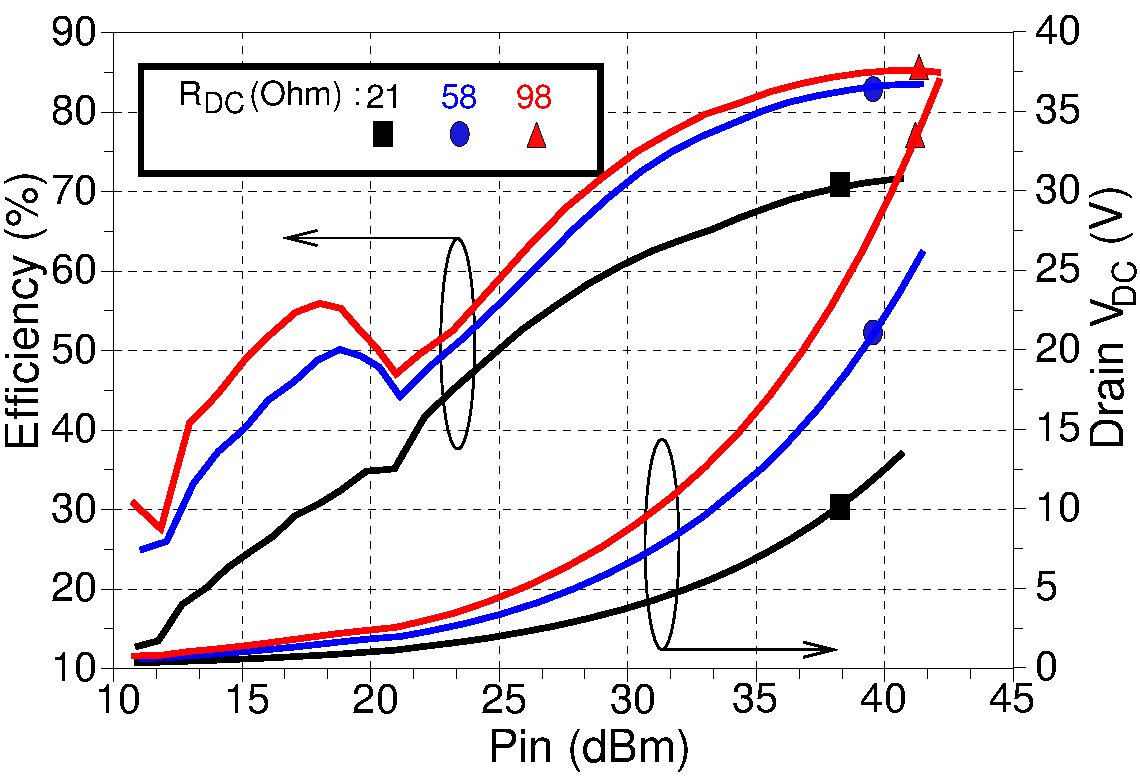
\includegraphics[width=3.4in]{pdf/13.pdf}
\caption{\hl{Conversion efficiency and drain DC output voltage versus input power for several DC drain resistor values. $V_{GS}=-4.4V$ and $Z_g(f_0)=\left(230+j10\right)\Omega$. The highest efficiency of 85\% is obtained at $P_{in}$=40\,dBm with a $V_{DC}$=30\,V.}}
\label{Rd_sweep_final}
\end{figure}


% === FIG : Zin
\begin{figure}[ht!]
\centering
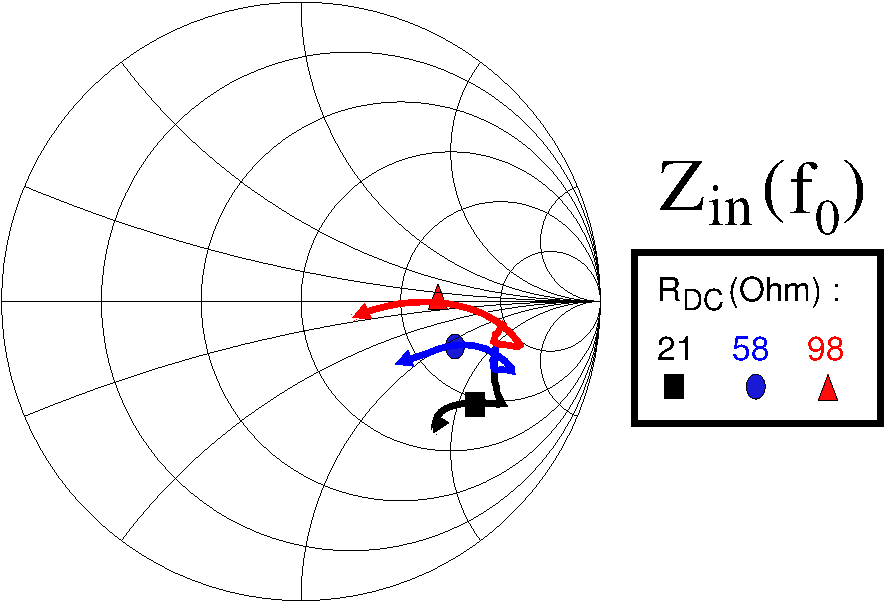
\includegraphics[width=3in]{pdf/14.pdf}
\caption{\hl{RF impedance at $f_0$ measured at the input (drain port) versus input power for several DC drain resistor values. $V_{GS}=-4.4V$ and $Z_g(f_0)=\left(230+j10\right)\Omega$.}}
\label{Rd_sweep_Zin}
\end{figure}



% ===================================================================================================================================
% ===================================================================================================================================
% \subsubsection{Sweeping \textbf{Vg} - the gate power supply}

Finally, the effect of the gate bias $V_{GS}$ on the rectifier efficiency, output voltage and input impedance was investigated. The gate impedance in this case was set for highest efficiency (230\,$\Omega$), and a DC load of 58\,$\Omega$ was selected in order to protect the transistor from high drain voltages that occur for the 98\,$\Omega$ load that corresponds to the highest efficiency. The measurements were performed for six different values of gate bias $V_{GS}$ as shown in Fig.~\ref{VG_sweep_final}. \hl{With $R_{DC}=58\Omega$,} a maximum efficiency of 83\% was obtained with the transistor biased deeply into the pinch-off region with $V_{GS}=-4.4$\,V, and a drop of only  3\% was measured for $V_{GS}=-3.5$\,V. Furthermore, the gate bias \hl{has a minimal impact} on the output DC voltage or on the drain impedance.


% === FIG : SWEEP VG
\begin{figure}[ht!]
\centering
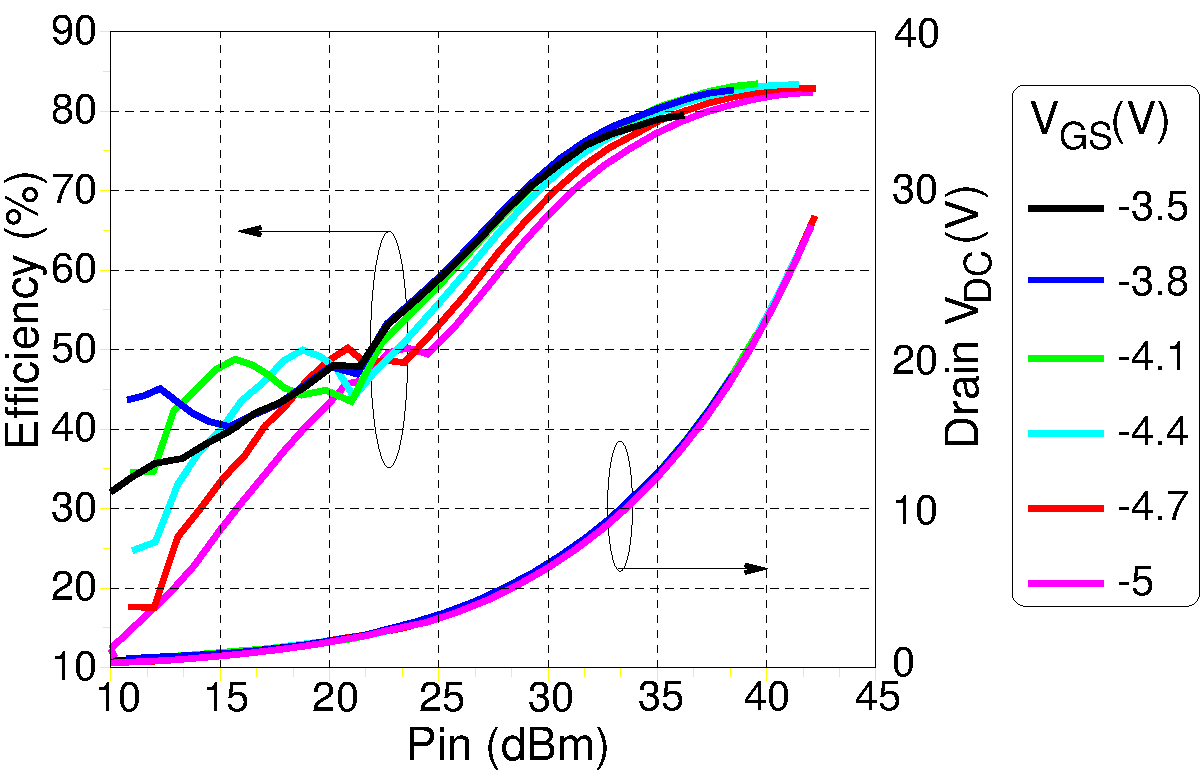
\includegraphics[width=3.4in]{pdf/15.pdf}
\caption{Measured conversion efficiency and drain DC voltage versus input power for several DC gate voltage biases. For this data, $R_{DC}=58\Omega$ and $Z_g(f_0)=\left(230+j10\right)\Omega$.}
\label{VG_sweep_final}
\end{figure}





% ===================================================================================================================================
% ===================================================================================================================================


% An example of a floating figure using the graphicx package.
% Note that \label must occur AFTER (or within) \caption.
% For figures, \caption should occur after the \includegraphics.
% Note that IEEEtran v1.7 and later has special internal code that
% is designed to preserve the operation of \label within \caption
% even when the captionsoff option is in effect. However, because
% of issues like this, it may be the safest practice to put all your
% \label just after \caption rather than within \caption{}.
%
% Reminder: the "draftcls" or "draftclsnofoot", not "draft", class
% option should be used if it is desired that the figures are to be
% displayed while in draft mode.
%
%\begin{figure}[!t]
%\centering
%\includegraphics[width=2.5in]{myfigure}
% where an .eps filename suffix will be assumed under latex, 
% and a .pdf suffix will be assumed for pdflatex; or what has been declared
% via \DeclareGraphicsExtensions.
%\caption{Simulation Results}
%\label{fig_sim}
%\end{figure}

% Note that IEEE typically puts floats only at the top, even when this
% results in a large percentage of a column being occupied by floats.


% An example of a double column floating figure using two subfigures.
% (The subfig.sty package must be loaded for this to work.)
% The subfigure \label commands are set within each subfloat command, the
% \label for the overall figure must come after \caption.
% \hfil must be used as a separator to get equal spacing.
% The subfigure.sty package works much the same way, except \subfigure is
% used instead of \subfloat.
%
%\begin{figure*}[!t]
%\centerline{\subfloat[Case I]\includegraphics[width=2.5in]{subfigcase1}%
%\label{fig_first_case}}
%\hfil
%\subfloat[Case II]{\includegraphics[width=2.5in]{subfigcase2}%
%\label{fig_second_case}}}
%\caption{Simulation results}
%\label{fig_sim}
%\end{figure*}
%
% Note that often IEEE papers with subfigures do not employ subfigure
% captions (using the optional argument to \subfloat), but instead will
% reference/describe all of them (a), (b), etc., within the main caption.


% An example of a floating table. Note that, for IEEE style tables, the 
% \caption command should come BEFORE the table. Table text will default to
% \footnotesize as IEEE normally uses this smaller font for tables.
% The \label must come after \caption as always.
%
%\begin{table}[!t]
%% increase table row spacing, adjust to taste
%\renewcommand{\arraystretch}{1.3}
% if using array.sty, it might be a good idea to tweak the value of
% \extrarowheight as needed to properly center the text within the cells
%\caption{An Example of a Table}
%\label{table_example}
%\centering
%% Some packages, such as MDW tools, offer better commands for making tables
%% than the plain LaTeX2e tabular which is used here.
%\begin{tabular}{|c||c|}
%\hline
%One & Two\\
%\hline
%Three & Four\\
%\hline
%\end{tabular}
%\end{table}


% Note that IEEE does not put floats in the very first column - or typically
% anywhere on the first page for that matter. Also, in-text middle ("here")
% positioning is not used. Most IEEE journals use top floats exclusively.
% Note that, LaTeX2e, unlike IEEE journals, places footnotes above bottom
% floats. This can be corrected via the \fnbelowfloat command of the
% stfloats package.



\section{Conclusion}
In summary, this paper addresses high-efficiency power rectifiers designed with harmonic terminations at the RF input, in analogy to high-efficiency power amplifier design with harmonic terminations at the output. The applications of such power rectifiers include wireless power beaming \cite{brown_rect2}, recycling power in high-power circuits \cite{asbeck} and ultra-fast switching integrated DC-DC converters with no magnetics \cite{4500dcdc}.

The theory for an ideal rectification element is based on Fourier analysis and establishes the basic design parameters such as the relationship between output DC resistance and impedance at the fundamental frequency at the rectifier input which optimizes efficiency. The analysis also predicts the time-domain waveforms at the terminals of the rectification element and the efficiency as a function of on-resistance and DC output resistance. Specific results are derived for class-C and class-F$^{-1}$ classes of operation, as they are defined for power amplifiers. These two cases are chosen for experimental validation with a 2.45\,GHz diode and 2.14\,GHz transistor rectifier, respectively. It is straightforward to repeat the derivation for other classes of operation, such as class-F as shown in detail in \cite{roberg_phd}.

The experimental results show that good agreement can be reached between theory and experiment with a Schottky-diode single-ended rectifier with finite class-C harmonic terminations, resulting in 72.8\% efficiency for input power levels in the mW range, intended for wireless power harvesting detailed in \cite{robergIMS2012,erezMTT2012}. A GaN pHEMT class-F$^{-1}$ power rectifier achieved 85\% efficiency with \hl{40}\,dBm input power across 98-\,$\Omega$ DC load \hl{with a DC output voltage $V_{DC}=30V$}. The efficiency and output voltage of the self-synchronous rectifier are shown to depend on the input power at the drain, the impedance at the gate port and the DC load at the output drain bias line, but not on the gate bias.

Time-domain large-signal measurements of a class-F$^{-1}$ power amplifier configured as a rectifier show that one can accomplish the same rectifier efficiency as the amplifier drain efficiency in self-synchronous mode without external gate RF drive. This is somewhat surprising, and to the best of our knowledge, the first time this type of high-efficiency rectifier has been demonstrated.



\section*{Acknowledgment}


%Dr. Reveryrand would like to acknowledge the funding by XLIM, Limoges, France. 
The authors would like to thank Dr. David Root and Dr. Jean-Pierre Teyssier at Agilent Technologies for the loan of the time-domain nonlinear measurement equipment and TriQuint Semiconductor for the donation of the transistors. 



% if have a single appendix:
%\appendix[Proof of the Zonklar Equations]
% or
%\appendix  % for no appendix heading
% do not use \section anymore after \appendix, only \section*
% is possibly needed

% use appendices with more than one appendix
% then use \section to start each appendix
% you must declare a \section before using any
% \subsection or using \label (\appendices by itself
% starts a section numbered zero.)
%

% ============================================
%\appendices
%\section{Proof of the First Zonklar Equation}
%Appendix one text goes here %\cite{Roberg2010}.

% you can choose not to have a title for an appendix
% if you want by leaving the argument blank
%\section{}
%Appendix two text goes here.


% use section* for acknowledgement
%\section*{Acknowledgment}


%The authors would like to thank D. Root for the loan of the SWAP. The SWAP that can ONLY be usefull in Boulder...


% Can use something like this to put references on a page
% by themselves when using endfloat and the captionsoff option.
\ifCLASSOPTIONcaptionsoff
  \newpage
\fi



% trigger a \newpage just before the given reference
% number - used to balance the columns on the last page
% adjust value as needed - may need to be readjusted if
% the document is modified later
%\IEEEtriggeratref{8}
% The "triggered" command can be changed if desired:
%\IEEEtriggercmd{\enlargethispage{-5in}}

% ====== REFERENCE SECTION

%\begin{thebibliography}{1}

% IEEEabrv,

\bibliographystyle{IEEEtran}
\bibliography{IEEEabrv,Bibliography}
%\end{thebibliography}
% biography section
% 
% If you have an EPS/PDF photo (graphicx package needed) extra braces are
% needed around the contents of the optional argument to biography to prevent
% the LaTeX parser from getting confused when it sees the complicated
% \includegraphics command within an optional argument. (You could create
% your own custom macro containing the \includegraphics command to make things
% simpler here.)
%\begin{biography}[{\includegraphics[width=1in,height=1.25in,clip,keepaspectratio]{mshell}}]{Michael Shell}
% or if you just want to reserve a space for a photo:

% ==== SWITCH OFF the BIO for submission
% ==== SWITCH OFF the BIO for submission


%% if you will not have a photo at all:
%\begin{IEEEbiographynophoto}{Ignacio Ramos}
%(S'12) received the B.S. degree in electrical engineering from the University of Illinois at Chicago in 2009, and is currently working toward the Ph.D. degree at the University of Colorado at Boulder. From 2009 to 2011, he was with the Power and Electronic Systems Department at Raytheon IDS, Sudbury, MA. His research interests include high-efficiency microwave power amplifiers, microwave DC/DC converters, radar systems, and wireless power transmission.
%\end{IEEEbiographynophoto}

%% insert where needed to balance the two columns on the last page with
%% biographies
%%\newpage

%\begin{IEEEbiographynophoto}{Jane Doe}
%Biography text here.
%\end{IEEEbiographynophoto}
% ==== SWITCH OFF the BIO for submission
% ==== SWITCH OFF the BIO for submission



% You can push biographies down or up by placing
% a \vfill before or after them. The appropriate
% use of \vfill depends on what kind of text is
% on the last page and whether or not the columns
% are being equalized.

\vfill

% Can be used to pull up biographies so that the bottom of the last one
% is flush with the other column.
%\enlargethispage{-5in}



% that's all folks
\end{document}